%Template para TCC CIC UFRGS
%Author: Lucas Schnorr (Adaptado para overleaf por Rubens dos Santos)

% exemplo genérico de uso da classe iiufrgs.cls
% $Id: iiufrgs.tex,v 1.1.1.1 2005/01/18 23:54:42 avila Exp $
% 
% This is an example file and is hereby explicitly put in the
% public domain.
% 
\documentclass[cic,tc]{iiufrgs}
% Para usar o modelo, deve-se informar o programa e o tipo de documento.
% Programas :
% *cic       -- Graduação em Ciência da Computação
% * ecp       -- Graduação em Ciência da Computação
% * ppgc      -- Programa de Pós Graduação em Computação
% * pgmigro   -- Programa de Pós Graduação em Microeletrônica
% 
% Tipos de Documento:
% * tc                -- Trabalhos de Conclusão (apenas cic e ecp)
% * diss ou mestrado  -- Dissertações de Mestrado (ppgc e pgmicro)
% * tese ou doutorado -- Teses de Doutorado (ppgc e pgmicro)
% * ti                -- Trabalho Individual (ppgc e pgmicro)
% 
% Outras Opções:
% * english    -- para textos em inglês
% * openright  -- Força início de capítulos em páginas ímpares (padrão da
% biblioteca)
% * oneside    -- Desliga frente-e-verso
% * nominatalocal -- Lê os dados da nominata do arquivo nominatalocal.def


% Use unicode
\usepackage[utf8]{inputenc}   % pacote para acentuação

% Necessário para incluir figuras
\usepackage{graphicx}         % pacote para importar figuras

\usepackage{times}            % pacote para usar fonte Adobe Times
% \usepackage{palatino}
% \usepackage{mathptmx}       % p/ usar fonte Adobe Times nas fórmulas

\usepackage[alf,abnt-emphasize=bf]{abntex2cite}	% pacote para usar citações abnt

% equações
\usepackage{amsmath}

% marks
\usepackage{amsfonts}

% 
% Informações gerais
% 
\title{Comparativo de Métricas Intrínsecas para Avaliação do Desempenho de Modelos em Open-Ended Tasks}

\author{Fa{\'e}}{Eduardo Dalm{\'a}s}
% alguns documentos podem ter varios autores:
% \author{Flaumann}{Frida Gutenberg}
% \author{Flaumann}{Klaus Gutenberg}

% orientador e co-orientador são opcionais (não diga isso pra eles :))
\advisor[Prof.~Dr.]{Balreira}{Dennis Giovani}

% a data deve ser a da defesa; se nao especificada, são gerados
% mes e ano correntes
% \date{maio}{2001}

% o local de realização do trabalho pode ser especificado (ex. para TCs)
% com o comando \location:
% \location{Itaquaquecetuba}{SP}

% itens individuais da nominata podem ser redefinidos com os comandos
% abaixo:
\renewcommand{\nominataReit}{Prof\textsuperscript{a}.~Marcia Cristina Bernardes Barbosa}
\renewcommand{\nominataReitname}{Reitora}
\renewcommand{\nominataPRCA}{Prof.~Pedro de Almeida Costa}
\renewcommand{\nominataPRCAname}{Vice-Reitor}
\renewcommand{\nominataPRAPG}{Prof\textsuperscript{a}.~N{\'a}dya Pesce da Silveira}
\renewcommand{\nominataPRAPGname}{Pr{\'o}-Reitora de Gradua{\c{c}}{\~a}o}
\renewcommand{\nominataDir}{Prof.~Luciano Paschoal Gaspary}
\renewcommand{\nominataDirname}{Diretor do Instituto de Inform{\'a}tica}
\renewcommand{\nominataCoord}{Prof.~{\'A}lvaro Freitas Moreira}
\renewcommand{\nominataCoordname}{Coordenador do Curso de Ciência da Computação}
\renewcommand{\nominataBibchefe}{Alexsander Borges Ribeiro}
\renewcommand{\nominataBibchefename}{Bibliotec{\'a}rio-chefe do Instituto de Inform{\'a}tica}

% A seguir são apresentados comandos específicos para alguns
% tipos de documentos.

% Relatório de Pesquisa [rp]:
% \rp{123}             % numero do rp
% \financ{CNPq, CAPES} % orgaos financiadores

% Trabalho Individual [ti]:
% \ti{123}     % numero do TI
% \ti[II]{456} % no caso de ser o segundo TI

% Monografias de Especialização [espec]:
% \espec{Redes e Sistemas Distribuídos}      % nome do curso
% \coord[Profa.~Dra.]{Weber}{Taisy da Silva} % coordenador do curso
% \dept{INA}                                 % departamento relacionado

% 
% palavras-chave
% iniciar todas com letras minúsculas, exceto no caso de abreviaturas
% 
\keyword{PLN}
\keyword{Open-ended Tasks}
\keyword{Métricas}

%\settowidth{\seclen}{1.10~}

% 
% inicio do documento
% 
\begin{document}

% folha de rosto
% às vezes é necessário redefinir algum comando logo antes de produzir
% a folha de rosto:
% \renewcommand{\coordname}{Coordenadora do Curso}
\maketitle

% dedicatoria
\clearpage
\begin{flushright}
    \mbox{}\vfill
    {\sffamily\itshape
      ``Adversity Is the First Path to Truth''\\}
    --- \textsc{Lord Byron}
\end{flushright}

% agradecimentos
\chapter*{Agradecimentos}
Aos meus amigos de Cacimbinhas, pela amizade verdadeira, pelo auxílio fornecido e por aguentarem os meus formulários intermináveis.

Para minha família, meu alicerce constante, por todo o amor, apoio e confiança ao longo dessa jornada que hoje concluo.

Para Lara, o amor da minha vida, pela paciência e incentivo incondicional nos momentos de felicidade e tristeza, sempre me apoiando e motivando não importando a dificuldade enfrentada.

Finalmente, ao professor Dennis Giovani Balreira, por sua orientação generosa, ensinamentos valiosos e por sempre acreditar em mim.

% resumo na língua do documento
\begin{abstract}
    \textit{Open-Ended Tasks} são tarefas que não possuem uma única solução específica. Elas possuem uma grande ligação com a área de Processamento de Linguagem Natural e são tópicos de pesquisa muito populares nos últimos anos. Contudo, a avaliação dessas tarefas é um processo muito complexo e muitas métricas já foram propostas ao longo dos anos em prol de solucionar esse problema. O presente trabalho tem como objetivo catalogar as métricas mais comumente utilizadas e analisar quais delas melhor se adéquam para as tarefas de Sumarização e \textit{Question-Answering}. Ao mesmo tempo, busca-se correlacionar os valores gerados pelas métricas com a forma de avaliação humana. Para a realização dos testes foram utilizados \textit{datasets} e modelos na linguagem portuguesa. As saídas obtidas foram avaliadas pelas métricas automatizadas selecionadas e por quatro participantes humanos diferentes. Finalmente, foi realizado o cálculo da correlação entre as avaliações humanas e automatizadas, e apontou-se que as métricas atuais possuem, no máximo, uma correlação mediana com a forma de julgamento humano. Fato esse que já havia sido apontado por outros trabalhos na área, contudo feito pela primeira vez em português. Esses resultados apontam para uma necessidade de novas métricas que melhor se correlacionem com a percepção humana. Ademais, é possível perceber que métricas baseadas em Modelos de Linguagem Pré-Treinados apresentam maior correlação com a forma de avaliação humana. Por fim, notamos a carência de bons \textit{datasets} desenvolvidos diretamente para a língua portuguesa, o que pode ter impactado negativamente os resultados obtidos.
\end{abstract}

% resumo na outra língua
% como parametros devem ser passados o titulo e as palavras-chave
% na outra língua, separadas por vírgulas
\begin{englishabstract}{Comparison of Intrinsic Metrics for Evaluating Model Performance in Open-Ended Tasks}{NLP. Open-ended Tasks. Metrics}
    Open-Ended Tasks are tasks that do not have a single specific solution. They are closely connected to the field of Natural Language Processing and have become highly popular research topics in recent years. However, evaluating these tasks is a very complex process, and many metrics have been proposed over the years in an attempt to address this issue. This work aims to catalog the most commonly used metrics and analyze which of them are best suited for Summarization and Question-Answering tasks. At the same time, it seeks to correlate the values generated by the metrics with human evaluation. For the experiments, datasets and models in the Portuguese language were used. The generated outputs were evaluated by the selected automated metrics and by four different human participants. Finally, the correlation between human and automated evaluations was calculated, revealing that current metrics exhibit, at best, a moderate correlation with human judgment. This fact was previously noted in other studies in the field, though it is being reported for the first time in Portuguese. These results highlight the need for new metrics that better correlate with human perception. Furthermore, it is evident that metrics based on Pretrained Language Models (PLMs) tend to show a higher correlation with human evaluation. Lastly, we observed a lack of high-quality datasets developed specifically for the Portuguese language, which may have negatively impacted the obtained results.
\end{englishabstract}

% lista de figuras
\listoffigures

% lista de tabelas
\listoftables

% lista de abreviaturas e siglas
% o parametro deve ser a abreviatura mais longa
\begin{listofabbrv}{METEOR}
    \item[BART] \textit{Bidirectional and Auto-Regressive Transformer}
    \item[BERT] \textit{Bidirecional Encoder Representations from Transformers}
    \item[BLEU] \textit{Bilingual Evaluation Understudy}
    % \item[BP] Penalidade por Brevidade
    \item[DL] \textit{Deep Learning}
    \item[GPT] \textit{Generative Pre-trained Transformer}
    \item[HyDE] \textit{Hypothetical Document Embeddings} 
    \item[IA] Inteligência Artificial
    \item[LLM] \textit{Large Language Model}
    \item[LSTM] \textit{Long Short-Term Memory}
    \item[METEOR] \textit{Metric for Evaluation of Translation with Explicit ORdering}
    \item[PLM] \textit{Pre-trained Language Model}
    \item[PLN] Processamento de Linguagem Natural
    \item[QA] \textit{Question-Answering}
    \item[RAG] \textit{Retrieval-Augmented Generation} 
    \item[ROUGE] \textit{Recall-Oriented Understudy for Gisting Evaluation}
    \item[RNN] \textit{Recurrent Neural Network}
    \item[Seq2Seq] \textit{Sequence to Sequence} 
    \item[T5] \textit{Text-To-Text Transfer Transformer}
    \item[TF-IDF] \textit{Term Frequency-Inverse Document Frequency}
    \item[WMD] \textit{Word Mover's Distance}
\end{listofabbrv}

% idem para a lista de símbolos
% \begin{listofsymbols}{$\alpha\beta\pi\omega$}
%     \item[$\sum{\frac{a}{b}}$] Somatório do produtório
%     \item[$\alpha\beta\pi\omega$] Fator de inconstância do resultado
% \end{listofsymbols}

% sumario
\tableofcontents

% aqui comeca o texto propriamente dito

% introducao
\chapter{Introdução}
Processamento de Linguagem Natural (PLN) é uma área de Inteligência Artificial (IA) que trabalha com a interpretação, análise, manipulação e classificação de textos redigidos em linguagem natural, isso é, linguagens utilizadas por seres humanos em suas comunicações, verbais ou escritas. A área de PLN, em muitas ocasiões, trata de problemas que não possuem uma única resposta considerada correta. Segundo \citet{burrows2015eras}, essas tarefas, denominadas \textit{Open-ended Tasks}, são significativamente mais complexas de serem verificadas e avaliadas, dada a dificuldade de compreensão da linguagem natural. O fato de não possuírem uma única resposta específica acaba impondo problemas às análises de desempenho de modelos que tentam abordar esse tipo de tarefa, não permitindo uma simples comparação direta de uma saídas com um resultado esperado.

Graças a essas características exclusivas, inúmeras técnicas e métricas já foram propostas a fim de permitir uma avaliação automatizada e padronizada do desempenho de modelos na resolução de tais problemas. Contudo, com mais e mais métricas sendo propostas, como o BERTScore \cite{bert-score} e o BARTScore \cite{yuan2021bartscore}, surge o questionamento sobre qual seria a técnica de avaliação mais adequada para cada problema, e como os valores propostos por cada métrica se assemelham à forma como um ser humano avaliaria a saída gerada.

\section{Objetivos}
Este trabalho busca mensurar a correlação entre diferentes métricas de avaliação automatizadas e a forma de julgamento humana, quando se tratando da avaliação do desempenho de modelos computacionais no âmbito de \textit{open-ended tasks}. No decorrer deste trabalho, discutiremos quais as métricas mais populares, como cada métrica se correlaciona com a forma de avaliação humana e quais os problemas enfrentados para chegarmos nesses resultados. 

\section{Organização do trabalho}
Este trabalho é dividido em seis capítulos. O Capítulo \ref{cap:conceitos fundamentais} apresenta os conceitos básicos necessários para o entendimento do trabalho. O Capítulo \ref{cap:trabalhos relacionados} aborda alguns trabalhos similares ao tema proposto. A seguir, no Capítulo \ref{cap:metodologia} se encontra a descrição geral dos passos e escolhas tomadas na realização do projeto. O Capítulo \ref{cap:validação} apresenta e discute os experimentos e seus resultados obtidos, seguidos por uma discussão. Finalmente, no Capítulo \ref{cap:conclusão} é apresentada a conclusão atingida, além de limitações apresentadas e possíveis trabalhos futuros.

\chapter{Conceitos Fundamentais}
\label{cap:conceitos fundamentais}
Neste capítulo, apresentaremos os conceitos básicos necessários para o entendimento do que será tratado mais a frente no trabalho. Mais especificamente, na \autoref{sec:PLN}, apresentaremos o conceito de Processamento de Linguagem Natural; na \autoref{sec:LLMs}, apresentaremos o conceito de Large Language Models; na \autoref{sec:openendedtasks}, trataremos o que é uma \textit{open-ended task}; na \autoref{sec:avaliação-int-x-ext}, abordaremos a diferença entre avaliação intrínseca e extrínseca; nas Seções \ref{sec:métricas baseadas em n-gramas} e \ref{sec:métricas baseadas em PLMs}, apresentaremos as métricas abordadas no trabalho; e na \autoref{sec:pearson}, discutiremos a correlação de pearson e seu uso nesta área de pesquisa.

\section{Processamento de Linguagem Natural}
\label{sec:PLN}
Processamento de Linguagem Natural (PLN) é um campo da Inteligência Artificial (IA) que trata da compreensão, interpretação, análise e geração da linguagem natural utilizada pelos seres humanos em suas comunicações. O campo atua na interseção entre as áreas de Ciência da Computação e Linguística. Ele faz uso de estudos realizados em ambas as áreas, como os ramos de Morfologia e a Semântica da Linguística, além de ramos como IA e Aprendizado de Máquina na Ciência da Computação. Durante seus anos de evolução, PLN também teve grande influência do campo da Estatística.

A área tem sua origem diretamente ligada à Computação. Desde a concepção dos primeiros computadores, já se sonhava com a ideia de que os mesmos conseguissem compreender a linguagem humana. Essa busca por máquinas inteligentes, capazes de se comunicar com os seres humanos já se via presente em Alan Turing, considerado por muitos como o pai da computação, quando o mesmo propôs o que hoje denominamos de Teste de Turing, em seu artigo \textit{Computing Machinery and Intelligence} \cite{alan1950a}. 

\subsection{Teste de Turing}
O Teste de \citet{alan1950a} tinha como objetivo avaliar a capacidade de uma máquina de se tornar indistinguível a um ser humano. Ele era composto de duas salas, dois humanos e uma máquina a ser testada. Durante o teste um humano assumiria o papel de juiz e ficaria sozinho em uma das salas. O outro humano ficaria junto da maquina na outra sala e ambos seriam categorizados como participantes A e B. O juiz poderia fazer perguntas aos integrantes da outra sala e teria como objetivo determinar qual dos dois participantes é o ser humano. Já o participante humano teria de convencer o juiz que ele é o ser humano, enquanto a máquina tenta enganar o juiz levando o mesmo a pensar que ela seria o ser humano. 

Apesar de suas falhas, como a facilidade de manipulação, esse teste foi muito importante para o desenvolvimento da área de PLN como um todo, trazendo luz à ideia de uma máquina que consiga entender e se comunicar com seres humanos.

\subsection{O Argumento do Quarto Chinês}
O Argumento do Quarto Chinês é um experimento proposto pelo filósofo John Searle em seu artigo \textit{Minds, Brains and Programs} \cite{searle1980minds} que busca questionar as pressuposições nas quais o Teste de Turing \cite{alan1950a} se baseia. Segundo Searle, um indivíduo trancado em uma sala, que não entende chinês, poderia manipular os símbolos da língua apenas seguindo instruções formais escritas em sua própria língua, de forma que um observador externo pensaria que ele compreende chinês. Isso é paralelo ao proposto por Turing, onde um computador poderia passar o teste sem realmente entender a linguagem humana, apenas seguindo um padrão pré-estabelecido de regras com que está familiarizado.

Esse argumento demonstra como, mesmo que uma máquina simule um comportamento humano, não é possível garantir que a mesma compreenda suas ações. Evidenciando assim, a dificuldade presente em avaliar a real capacidade de uma máquina executando tarefas humanas.

% \section{Primórdios de PLN}
% \label{sec:modelos clássicos}
% \subsection{Modelos Baseados em Regras}
% Os primeiros trabalhos na área de PLN faziam uso de modelos baseados em regras. Tais modelos, como é o caso do Chatbot ELIZA \cite{weizenbaum1966eliza}, funcionavam apenas com casamento de padrões e regras pré-estabelecidas. Isso tornava a comunicação rígida e inflexível, muitas vezes gerando respostas que não condiziam com o estado da conversa.

% Esses modelos utilizavam de um conjunto predefinido de regras e padrões linguísticos para analisar, interpretar e gerar texto. Modelos desse tipo apresentavam problemas na sua produção e escalonamento, afinal, cada novo comportamento esperado precisava ser primeiro traduzido para uma regra e somente posteriormente implementado, o que requer um grande conhecimento de padrões linguísticos e muito tempo de dedicação. Além disso, novas regras podem acabar interferindo com regras anteriores, o que dificulta ainda mais o escalonamento de projetos.

% Os maiores problemas presentes em modelos baseados em regras é a inflexibilidade dos mesmos, isso é, se o modelo recebe algum texto que não foi tratado em sua estrutura de regras, ele não saberá como gerar uma reposta, muitas vezes tendo que retornar algum texto padrão, como: "Desculpe, não consigo te ajudar com isso". Esse comportamento demonstra como modelos baseados em regras, assim como a pessoa no quarto chinês, não conseguem realmente compreender o texto, mas apenas seguir um conjunto de padrões aos quais tem acesso. Tal comportamento, acompanhado de um conjunto perfeito de regras, pode até permitir que um modelo simule a forma de agir humana, mas não permite que o mesmo obtenha uma compreensão real da linguagem natural. A inflexibilidade também se torna muito problemática quando trabalhamos com linguagens naturais, pois elas estão em constante evolução, necessitando que os modelos sejam constantemente atualizados para evitar que fiquem obsoletos.

% \subsection{Modelos Estatísticos}
% Modelos Estatísticos começaram a surgir por volta de 1985 com o objetivo de facilitar e agilizar o desenvolvimento de novos modelos. A ideia principal é fazer com que o próprio modelo, com base em \textit{datasets} e técnicas probabilísticas, aprenda os padrões e relações entre os dados linguísticos. Alguns exemplos de modelos estatísticos propostos são: $n$-gramas \cite{shannon1948mathematical} e TF-IDF \cite{sparck1972statistical}.

% Apesar de facilitar a produção de novos modelos, já que não se faz mais necessária a geração manual de regras para cada caso a ser tratado, modelos estatísticos ainda sofrem com problemas de flexibilidade. Afinal, casos que não estão presentes nos dados de treinamento não serão tratados corretamente pelos modelos. 

% Os maiores problemas de modelos estatísticos são em grande partes compartilhados com modelos baseados em regras. Casos não vistos nos dados de treino não gerarão boas respostas, o que, com a evolução constante das linguagens naturais, torna os modelos rapidamente obsoletos quando não atualizados. Além disso, muitos dos modelos necessitam de uma grande quantidade de dados corretos e bem catalogados, o que exige um grande trabalho de coleta e tratamento de dados.

% \subsection{Deep Learning e Word Embeddings}
% Com os avanços em poder computacional e a disponibilidade de grandes volumes de dados durante a década de 2010, técnicas baseadas em \textit{Deep Learning} (DL) se estabeleceram como nova norma na área de PLN. Esses modelos eram capazes de inferir representações mais complexas e contextuais da linguagem.

% A popularização das \textit{word embeddings}, representações vetoriais densas que capturam semelhanças semânticas entre palavras, foi um marco importante na história da área. Técnicas como o Word2Vec \cite{mikolov2013distributed} possibilitaram a representação de palavras em um espaço vetorial contínuo, permitindo modelagens eficazes de relações semânticas e sintáticas. Modelos de DL, como RNNs e LSTMs, fizeram amplo uso dessas novas técnicas, buscando tratar tarefas sequenciais, como tradução automática e análise de sentimentos.

\section{Large Language Models}
\label{sec:LLMs}
%MUDADO
\textit{Large Language Models} (LLMs), são sistemas de inteligência artificial treinados com enormes quantidades de texto para aprender padrões linguísticos complexos. Esses modelos são baseados em arquiteturas de redes neurais profundas, como o \textit{Transformer}, quer serão abordados na \autoref{sec:transformers}. Eles se destacam por sua capacidade de compreender e gerar linguagem natural de maneira coerente e contextualizada. Eles vêm sendo utilizados em uma ampla gama de aplicações, incluindo tradução automática, sumarização e \textit{question-answering}.

%MUDADO
Uma das características desse tipo de modelo é o número extremamente elevado de parâmetros o que lhes confere uma grande expressividade e capacidade de generalização. Ademais, uma característica comumente apresentada por LLMs é a capacidade de realizar tarefas complexas com pouco ou nenhum ajuste específico, mesmo quando não foram treinados diretamente para elas.

\subsection{Transformers}
\label{sec:transformers}
%MUDADO
\textit{Transformers} é um tipo de arquitetura baseada no mecanismo de atenção proposto por \citet{vaswani2023attentionneed}, que permite aos modelos uma captura de relações complexas em sequências de texto. Modelos baseados nessa arquitetura influenciaram profundamente o mundo de PLN e ainda são muito utilizados tanto para compreensão, quanto para geração de textos em linguagem natural.

%MUDADO
O primeiro modelo Transformer \cite{vaswani2023attentionneed} foi proposto para a tarefa de tradução automática e era um modelo \textit{Sequence to Sequence} (Seq2Seq), isto é, modelava o problema com uma sequência de entrada e outra de saída. Por ser Seq2Seq, o Transformer possuía uma parte \textit{encoder} e outra parte \textit{decoder}. Diversos modelos posteriores ao Transformer original usam combinações de \textit{enconder-only} (BERT), \textit{decoder-only} (GPT) ou \textit{encoder-decoder} (T5).

\subsection{BERT}
BERT \cite{devlin2019bert} é um modelo de linguagem que redefiniu a forma como tratamos modelos, graças a sua capacidade de interpretar o contexto de uma palavra observando não somente o que lhe precede, como também o que lhe procede. Essa diferença na maneira de contextualização da palavra é o que lhe dá o nome de \textit{Bidirectional Encoder Representations from Transformers} (Representações Bidirecionais de Codificadores a partir de Transformers).

Diferentemente do GPT \cite{radford2018improving} e do T5 \cite{raffel2020exploring}, BERT utiliza apenas a parte de \textit{encoding} dos Transformers, afinal sua função primária é interpretar o texto. Através desse novo modelo, foi possível capturar nuances mais sutis do uso da palavra em dado contexto, gerando melhorias expressivas em diversas tarefas de PLN, como reconhecimento de entidades nomeadas e inferência textual. A partir do BERT também foram desenvolvidas diferentes aplicações, como o BERTScore \cite{bert-score}, uma métrica de avaliação que será tratada na \autoref{sec:bert-score}.

\section{Open-ended Tasks}
\label{sec:openendedtasks}
Segundo \citet{jastrzkebowska2021opening}, \textit{Open-ended tasks} são tarefas projetadas para que possam existir mais de uma resposta correta ou possam ser respondidas de mais de uma maneira. Elas são primariamente subjetivas e permitem diferentes interpretações e soluções. Esse tipo de tarefa está comumente presente em áreas que exigem criatividade e pensamento crítico. Na linguística, por exemplo, a produção de texto pode ser considerada uma tarefa de natureza aberta. 

O campo de PLN, por trabalhar diretamente com a linguagem humana, uma entidade volátil e repleta de nuances, tem grande ligação com \textit{open-ended tasks}. Afinal, quando se trabalha com comunicação, não existe uma única maneira de expressar uma ideia ou um conceito. Alguns exemplos de \textit{open-ended tasks} comumente presentes em trabalhos no campo de PLN são: sumarização, tradução automática e \textit{question-answering}, dois dos quais serão expandidos nesse trabalho.

Diferentemente de \textit{closed-ended tasks}, que trabalham com problemas que possuem uma única resposta objetiva e verificável, \textit{open-ended tasks} apresentam grandes dificuldades na validação e avaliação de uma resposta. Isso acontece pois não é possível rejeitar toda saída que difira da resposta esperada, já que não existe uma única resposta objetivamente correta. Por esses motivos, inúmeras técnicas já foram propostas a fim de tentar sanar esse problema estrutural desse tipo de tarefas. Contudo, ainda não existe um consenso sobre qual a melhor maneira de avaliar as saídas geradas.

Nas próximas subseções, apresentaremos as tarefas abordadas neste trabalho.

\subsection{Sumarização}
\label{sec:summ}
Sumarização consiste na produção de resumos dado um texto base. Ela é considerada uma \textit{open-ended task} por não possuir uma única maneira correta de ser realizada. Isso acontece pois um texto pode ser resumido de inúmeras maneiras diferentes, não possuindo um único jeito correto. 

Sumários podem variar devido a abordagens extrativas ou abstrativas, uso de sinônimos ou figuras de linguagem, escolha de tornar o resumo mais breve e focado no cerne do texto ou mais comprido encapsulando mais pontos do texto base. E, mesmo com essas divergências, todos podem ser igualmente bons.

\subsection{Question-Answering}
\label{sec:qa}
\textit{Quetion-answering} consiste na geração de respostas para perguntas. Essa tarefa é primariamente \textit{open-ended} por, assim como a sumarização, não possuir uma única resposta correta, podendo variar, embora menos, em objetividade ou através do uso de instrumentos de linguagem. 

Quando trabalhamos com \textit{question-answering} é muito comum, juntamente à pergunta, passarmos um contexto à LLM, que servirá como base para a resposta. Normalmente, quando tratamos esse tipo de tarefa, o fazemos através de uma de duas abordagens distintas, sendo uma extrativa, que busca apenas extrair a resposta diretamente do contexto, e outra abstrativa, buscando abstrair o significado do contexto para depois gerar a sua resposta. Essas diferentes abordagens fazem com que, apesar de ser originalmente uma \textit{open-ended task}, essa tarefa possa, em muitos casos, ser considerada \textit{close-ended}, principalmente quando focamos em abordagens extrativas.

\section{Avaliação Intrínseca x Avaliação Extrínseca}
\label{sec:avaliação-int-x-ext}
A avaliação intrínseca e a avaliação extrínseca são duas abordagens distintas para medir a qualidade de sistemas. Enquanto a avaliação intrínseca avalia a saída de um sistema com critérios e métrica pré-estabelecidas, a avaliação extrínseca foca em avaliar a saída dentro do contexto real de uso. Em suma, a avaliação intrínseca é uma avaliação mais objetiva e generalista, já a avaliação extrínseca é mais subjetiva e especializada. Essas características fazem da avaliação intrínseca uma tarefa facilmente padronizada e automatizada. 

Quando trabalhamos com análise de um resultado de um modelo, o ideal sempre é termos ambas avaliações. Contudo, nem sempre é tão fácil executar uma avaliação extrínseca, por isso muitos trabalhos focam nos resultados palpáveis da avaliação intrínseca. 

No entanto, no âmbito de \textit{open-ended tasks}, mesmo uma avaliação intrínseca já é extremamente complexa de ser feita. Afinal, não temos uma distinção binária de se um resultado é certo ou não. Uma saída pode ser parcialmente correta, duas saídas distintas podem estar corretas, dentre outros problemas já comentados que se fazem presentes em \textit{open-ended tasks}. Por tal motivo, muitas métricas já foram propostas em prol de realizar análises intrínsecas, mas ainda não se tem uma métrica definitiva para cada situação.

Nas próximas seções, discutiremos algumas das principais métricas utilizadas para avaliação intrínseca nos dias atuais.

\section{Métricas baseadas em N-Gramas}
\label{sec:métricas baseadas em n-gramas}
As métricas baseadas em n-grama são o primeiro tipo de métricas intrínsecas automatizadas focadas em \textit{open-ended tasks}. Essas métricas fazem uso do conceito estatístico de $n$-gramas \cite{shannon1948mathematical} para avaliar a fidelidade de um texto, comparando o texto gerado a um (ou mais) textos referência.

Essas métricas estão longe de serem perfeitas, principalmente devido à baixa capacidade de capturar semântica e sensibilidade quanto a variação lexical. Assim, esse tipo de métrica avalia apenas a sobreposição de palavras, o que por si só não permite um entendimento do contexto semântico da frase, ou reconhecimento de palavras sinônimas. 
%MUDADO
Um exemplo disso pode ser visto na \autoref{fig:problema-ngrama}, onde um humano conseguiria facilmente perceber que os textos falam a mesma coisa, enquanto esse tipo de métrica sofreria dado o uso de sinônimos.

%MUDADO
\begin{figure}[htbp]
    \caption{Exemplo de problema nas técnicas baseadas em $n$-gramas, onde um ser humano conseguiria facilmente reconhecer o correto no caso.}
    \begin{center}
    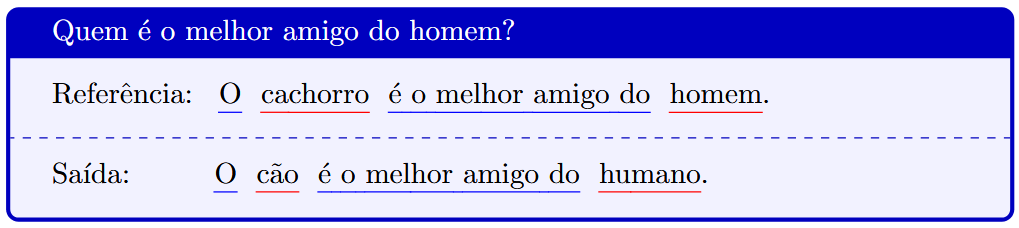
\includegraphics[width=\textwidth]{Figures/sinonimos-problema.png}
    \end{center}
    \legend{Fonte: O autor.}
    \label{fig:problema-ngrama}
\end{figure}

Mas nem tudo são espinhos, alguns dos pontos positivos dessas métricas incluem: fácil implementação, objetividade e reprodutibilidade. Isso permite que essas técnicas sejam facilmente reproduzidas e sirvam como uma comparação objetiva do desempenho de dois modelos diferentes. Essas características fazem com que, apesar de seus problemas, essas métricas continuem sendo muito utilizadas até os dias atuais, permitindo a comparação de novos modelos com modelos antigos. 

As próximas subseções apresentam algumas destas principais métricas.

\subsection{ROUGE}
ROUGE \cite{lin2004rouge} é uma das técnicas mais utilizadas desde a sua concepção, possuindo uma gama de versões e permitindo uma análise objetiva de forma rápida e prática. Dentre as diferentes versões do ROUGE \cite{lin2004rouge} se destacam ROUGE-N e ROUGE-L. O ROUGE-N foca em n-gramas, podendo eles serem unigramas, ROUGE-1, ou bigramas, ROUGE-2, e assim por diante. Já o ROUGE-L foca na maior subsequência compartilhada, isso é, no maior conjunto de palavras sequenciais em ordem compartilhado entre os textos. Os cálculos dos valores de ROUGE-N (Equações \ref{eq:rouge-n-1} e \ref{eq:rouge-n-2}) e ROUGE-L (Equações \ref{eq:rouge-l1} e \ref{eq:rouge-l2}) são expressos abaixo.

\begin{equation}
    \label{eq:rouge-n-1}
    \text{Match}(\text{g}) =
    \min\left(\text{count}_{\text{ref}}(\text{g}), \text{count}_{\text{pred}}(\text{g}) \right)
\end{equation}

\begin{equation}
    \label{eq:rouge-n-2}
    \text{ROUGE-N} = 
    \frac{
    \sum_{\text{n-gram} \in ref}
    \text{Match}(\text{n-gram})
    }{
    \sum_{\text{n-gram} \in ref} \text{count}_{\text{ref}}(\text{n-gram})
    }
\end{equation}

\begin{equation}
    \label{eq:rouge-l1} 
    R_{\text{LCS}} = \frac{ \text{LCS}(ref, pred) }{ ||ref|| }
    \quad\text{e}\quad
    P_{\text{LCS}} = \frac{ \text{LCS}(ref, pred) }{ ||pred|| }
\end{equation}

\begin{equation}
    \label{eq:rouge-l2}
    \text{ROUGE-L} =
    \frac{ 2 \cdot R_{\text{LCS}} \cdot P_{\text{LCS}} }
    { R_{\text{LCS}} + \cdot P_{\text{LCS}} }
\end{equation}

Apesar de suas grandes limitações, como a incapacidade de reconhecer sinônimos, ROUGE se manteve popular graças à sua simplicidade e à possibilidade de comparação de novos modelos com modelos antigos. Isso se da pelo fato de já existir grande quantidade de trabalhos que fizeram uso dessa métrica para a avaliação de seus modelos.

\subsection{BLEU}
O BLEU \cite{papineni2002bleu} é uma métrica automática que tem como foco avaliar a qualidade de traduções automáticas. Ela trabalha comparando o texto gerado com textos referências elaborados por humanos, sendo a primeira métrica automatizada a utilizar n-gramas de forma sistemática, influenciando fortemente o campo como um todo.

Para chegar em sua nota, BLEU calcula a precisão dos $n$-gramas de um a quatro, utilizando um sistema que limita a contagem de cada n-grama baseado no número de vezes que o mesmo se encontra no texto referência (Equações \ref{eq:precisionBLEU-1} e \ref{eq:precisionBLEU-2}). Além disso, a métrica também calcula uma penalidade por brevidade (BP) (\autoref{eq:penalidadeBLEU}), já que acredita que textos muito curtos tendem a ter uma maior sobreposição de palavras.

\begin{equation}
    \label{eq:precisionBLEU-1}
    \text{Match}(\text{g}) =
    \min\left(\text{count}_{\text{pred}}(\text{g}), \text{count}_{\text{ref}}(\text{g}) \right)
\end{equation}

\begin{equation}
    \label{eq:precisionBLEU-2}
    P_n = \frac{
    \sum_{\text{n-gram} \in pred} \text{Match}(\text{n-gram})
    }{
    \sum_{\text{n-gram} \in pred} \text{count}_{pred}(\text{n-gram})
    }
\end{equation}

\begin{equation}
    \label{eq:penalidadeBLEU}
    \text{BP} = 
    \begin{cases}
        1, & \text{se } ||pred|| > ||ref|| \\
        e^{1 - \frac{||ref||}{||pred||}}, & \text{se } ||pred|| \leq ||ref||
    \end{cases}
\end{equation}

O score final é obtido através de uma combinação das precisões calculadas com a penalidade por brevidade. Esse cálculo é feito segundo o descrito na \autoref{eq:BLEUval}, com $w_n$ sendo definido como $\frac{1}{N}$ no trabalho original.

\begin{equation}
    \label{eq:BLEUval}
    \text{BLEU} = \text{BP} \times \exp\left( \sum_{n=1}^N w_n \log P_n \right)
\end{equation}

Embora desenvolvida primariamente para tradução automática, BLEU é uma das métricas mais utilizada para avaliação de qualquer \textit{open-ended task} e se tornou inspiração para várias outras técnicas que buscam sanar algumas de suas falhas.

\subsection{METEOR}
METEOR \cite{banerjee2005meteor} é uma técnica que teve grande inspiração em BLEU, buscando remediar alguns de seus problemas. Ela, assim como as demais, utiliza $n$-gramas para realizar o alinhamento das palavras entre o texto gerado e o texto referência. Contudo, diferentemente das técnicas supracitadas, METEOR considera mais do que apenas correspondências exatas, também permitindo sinônimos, variações morfológicas e correspondências de raiz. Essa permite o reconhecimento de similaridades de sentido mesmo em palavras que não são expressamente iguais.

%\missingfigure{METEOR funcionamento}

Assim como o BLEU, o METEOR também faz uso de uma penalidade. Todavia, contrário ao que acontece em seu antecessor, essa penalidade não é baseada na brevidade, mas sim no ordenamento das palavras. Dessa forma, a métrica consegue reduzir o \textit{score} de um texto gerado que possua as palavras corretas, mas desordenadas. Para o cálculo da métrica em si, o METEOR faz uso de ambos precisão e \textit{recall}, posteriormente combinando-os através de uma média harmônica para calcular o \textit{F1-Score}, o que possibilita uma avaliação mais justa, especialmente em textos curtos. Nas Equações \ref{eq:METEORp}, \ref{eq:METEORpenalidade} e \ref{eq:METEORval}, pode ser visto o cálculo utilizado pela métrica para chegar em seu valor.

\begin{equation}
    \label{eq:METEORp}
    P = \frac{\text{\#1-grams}}{||pred||}, \quad R = \frac{\text{\#1-grams}}{||ref||} \quad e \quad F_{\alpha} = \frac{P \cdot R}{\alpha \cdot P + (1 - \alpha) \cdot R}
\end{equation}

\begin{equation}
    \label{eq:METEORpenalidade}
    \text{Penalidade} = \gamma \cdot \left(\frac{\text{\#chunks}}{\text{\#1-grams}}\right)^{\beta}
\end{equation}

\begin{equation}
    \label{eq:METEORval}
    \text{METEOR} = (1 - \text{Penalidade}) \cdot F_{\alpha}
\end{equation}

Com $\alpha$, $\beta$ e $\gamma$ sendo variáveis ajustáveis que foram originalmente definidas como 0.90, 3.0 e 0.5, respectivamente.

Apesar de tratar algumas das falhas de seus predecessores, como os problemas com sinônimos e palavras fora de ordem, o METEOR ainda apresenta diversos problemas, não conseguindo captar de forma profunda as nuances semânticas entre os textos.

\section{Métricas baseadas em Modelos de Linguagem Pré-Treinados}
\label{sec:métricas baseadas em PLMs}
Métricas baseadas e Modelos de Linguagem Pré-Treinados (PLMs) tiveram origem junto da emergência e ascensão das LLMs. Essas métricas utilizam modelos para fazer o cruzamento entre o texto gerado e o texto referência. Isso é realizado através do cálculo da Similaridade de Cossenos entre as \textit{embeddings} contextuais de ambos os textos.

Algumas desvantagens desse tipo de métrica incluem a dependência de bons modelos pré-treinados, alto custo computacional e sensibilidade ao idioma e domínio do modelo utilizado. Isso se dá pela necessidade de utilização de modelos, como o BERT \cite{devlin2019bert}, para fins de realização das \textit{embeddings} contextuais, ou seja, a qualidade da métrica está diretamente conectada à qualidade do modelo utilizado. Além disso, o uso de modelos para análise torna o processo mais lento e custoso.

Já as vantagens dessas métricas são: capacidade de análise semântica e avaliação contextualizada. Graças aos \textit{embeddings} contextuais, diferentemente das métricas baseadas em $n$-gramas \cite{shannon1948mathematical}, essas métricas conseguem capturar a similaridade semânticas entre os textos, mesmo com o uso de instrumentos linguísticos, como sinônimos e paráfrases. Essas capacidades fazem com que tais métricas sejam consideradas estado da arte quando se tratando de avaliação intrínseca.

\subsection{BERTScore}
\label{sec:bert-score}
BERTScore \cite{bert-score} foi uma das primeiras métricas baseadas em PLMs e o primeiro trabalho amplamente citado que popularizou e sistematizou o uso desse tipo de métricas. O BERTScore faz uso das \textit{embeddings} contextuais de modelos BERT para comparar textos gerados com textos referência nos mais diversos tipos de tarefas abertas. 

O pipeline do BERTScore (\autoref{fig:bert}) começa com a conversão de cada palavra nos textos para vetores de \textit{embeddings} contextuais, que são obtidos das camadas internas do modelo BERT escolhido. Após isso, é calculada a similaridade de cosseno entre cada vetor do texto gerado e do texto referência, buscando alinhar as palavras mais semanticamente similares entre os dois textos. 

\begin{figure}[htbp]
    \centering
    \caption{\textit{Pipeline} do BERTScore com as etapas de \textit{embedding} contextual dos textos analisados e o cálculo da similaridade de cosseno das \textit{embeddings} geradas.}
    \vspace{4mm}
    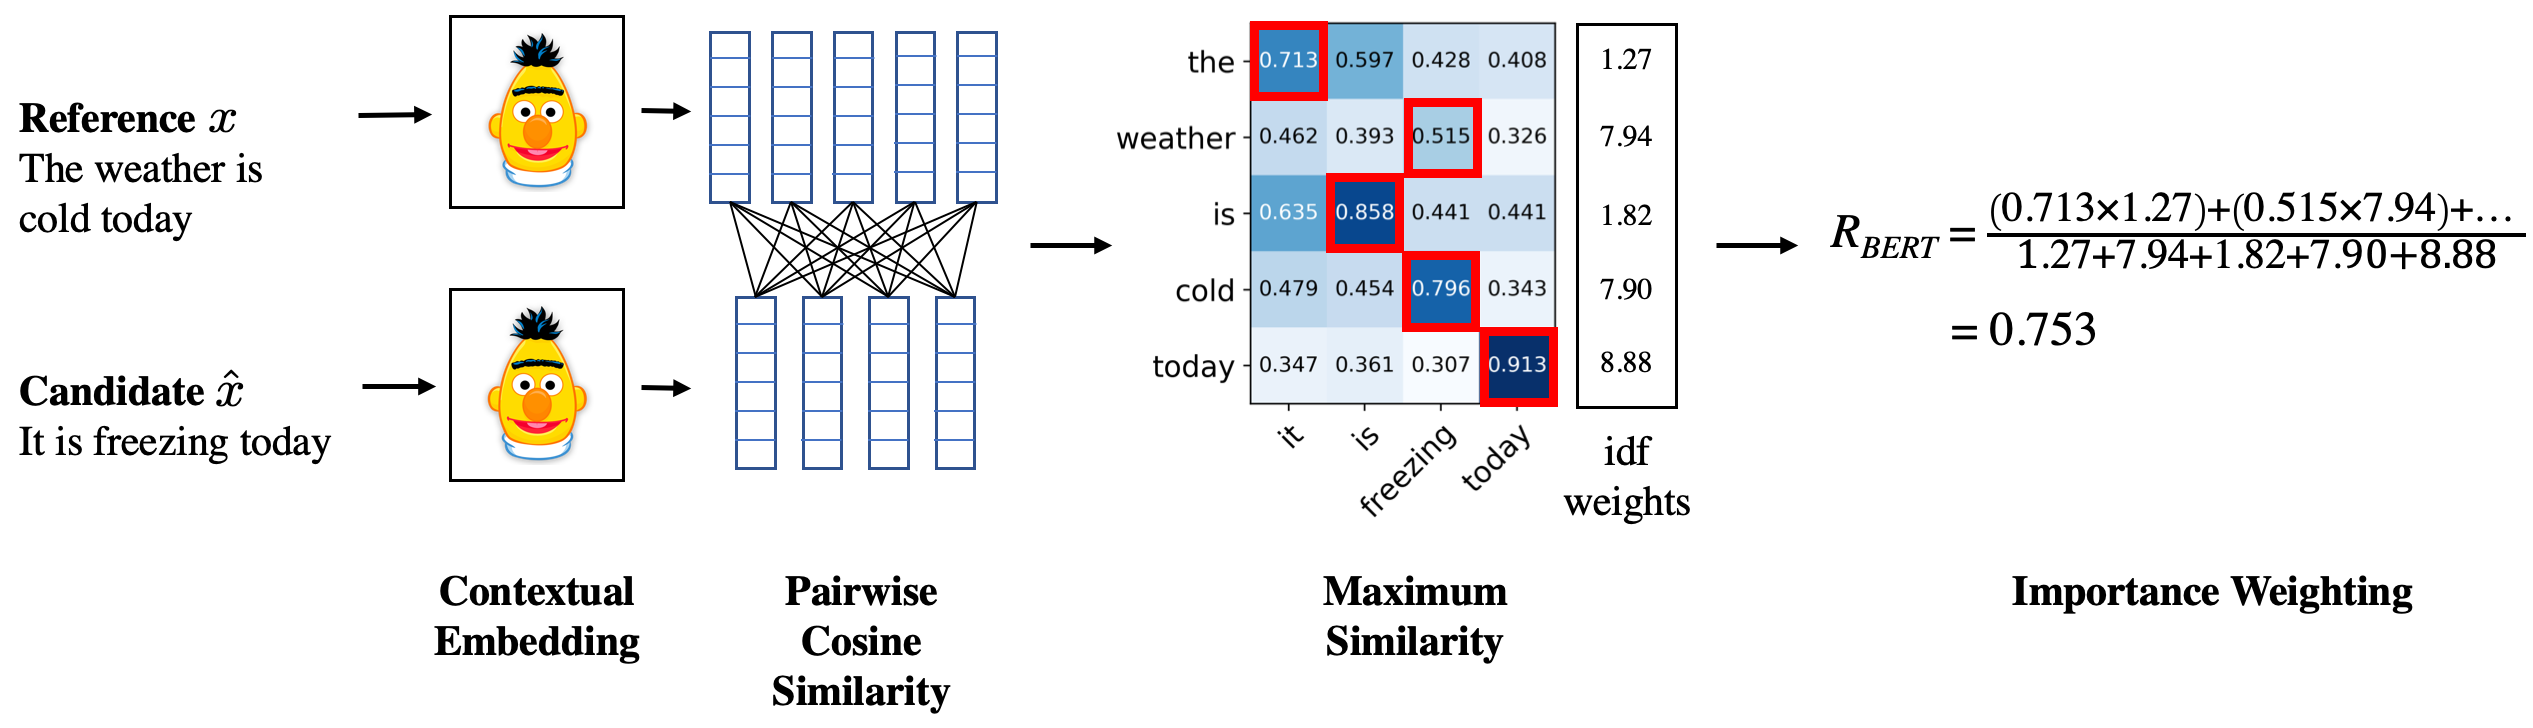
\includegraphics[width=\textwidth]{Figures/bert_score.png}
    \legend{Exemplo extraído de \citet{bert-score}.}
    \label{fig:bert}
\end{figure}

A similaridade de cosseno é calculada em ambos os sentidos, gerando assim os valores de precisão (\autoref{eq:BERTScore-p}) e \textit{recall} (\autoref{eq:BERTScore-r}). Ademais, o \textit{F1-Score} é calculado através de uma média harmônica entre os valores de precisão e \textit{recall} (\autoref{eq:BERTScore-f1}), representando um equilíbrio entre os dois valores e capturando de forma mais complexa a similaridade semântica entre os textos.

\begin{equation}
    \label{eq:BERTScore-p}
    P = \frac{1}{||pred||} \sum_{i=1}^{||pred||} \max_{j \in [1, ||ref||]} \text{Sim}(\text{pred}_i, \text{ref}_j)
\end{equation}

\begin{equation}
    \label{eq:BERTScore-r}
    R = \frac{1}{||ref||} \sum_{j=1}^{||ref||} \max_{i \in [1, ||pred||]} \text{Sim}(\text{pred}_i, \text{ref}_j)
\end{equation}

\begin{equation}
    \label{eq:BERTScore-f1}
    F_1 = \frac{2 \cdot P \cdot R}{P + R}
\end{equation}

\subsection{BARTScore}
BARTScore \cite{yuan2021bartscore} é uma métrica automática baseada em modelos BART \cite{lewis2019bart}. Diferentemente do BERTScore, essa métrica não faz uso de similaridade vetorial, mas sim da probabilidade logarítmica de que, dado um texto base, o modelo BART utilizado gere a saída analisada. Essa abordagem permite que o BARTScore calcule a qualidade da saída com base no que o modelo aprendeu sobre linguagem natural.

\subsection{MoverScore}
MoverScore \cite{zhao2019moverscore} foi uma das primeiras métricas baseadas em PLMs, surgindo junto do BERTScore e ajudando a popularizar esse tipo de abordagem. A métrica foi desenvolvida com o objetivo de superar as limitações de métricas tradicionais, como BLEU e ROUGE. Ela inovou o campo de avaliação automática ao utilizar \textit{embeddings} contextuais e técnicas de transporte ótimo como método de comparação de textos.

O seu funcionamento se baseia no conceito de \textit{Word Mover's Distance} (WMD) \cite{kusner2015word}, que calcula o menor custo necessário para transformar uma palavra em outra, dado a distância vetorial entre suas \textit{embeddings} contextuais% (\autoref{eq:MoverScore-WDM})
. Primeiramente, as palavras de ambos os textos são transformadas em suas respectivas \textit{embeddings} contextuais, dado o PLM utilizado. Além disso, cada palavra recebe um peso de importância, derivado do valor do TF-IDF \cite{sparck1972statistical}% (\autoref{eq:MoverScore-tfidf})
. Após isso, é calculado o custo mínimo de transporte para alinhar os vetores das palavras de cada texto através de WMD. Esse cálculo leva em consideração tanto a distância vetorial entre as \textit{embeddings} contextuais, quanto o peso de importância calculado para a palavra% (\autoref{eq:MoverScore-val})
. Assim, gerando um resultado que encapsula o esforço semântico necessário para transformar um texto em outro.

% \begin{equation}
%     \label{eq:MoverScore-WDM}
%     d_{ij} = 1 - \frac{\mathbf{h}_i \cdot \mathbf{r}_j}{\|\mathbf{h}_i\| \|\mathbf{r}_j\|}
% \end{equation}
% \begin{equation}
%     \label{eq:MoverScore-tfidf}
%     \text{idf}_H = \{w_1^h, \ldots, w_m^h\} \quad e \quad \text{idf}_R = \{w_1^r, \ldots, w_n^r\}
% \end{equation}
% \begin{equation}
%     \label{eq:MoverScore-val}
%     \text{MoverScore} = \min_{T \in \mathcal{U}(w^h, w^r)} \sum_{i=1}^{m} \sum_{j=1}^{n} T_{ij} \cdot d_{ij}
% \end{equation}

\section{Correlação de Pearson}
\label{sec:pearson}
A correlação de Pearson é uma medida estatística amplamente empregada quando se deseja quantificar as relações lineares entre duas variáveis numéricas. Essa correlação busca mensurar de forma direta o quanto variações em uma variável acompanham variações em outra.

Essa medida é muito utilizada em trabalhos no campo de PLN para mensurar a correlação entre métricas automatizadas e avaliações humanas, como é o caso do trabalho SummEval \cite{fabbri2021summeval} que será abordado na \autoref{sec:summeval}. Caso os valores gerados pelas métricas tendam a espelhar o comportamento observado nas análises humanas, espera-se um coeficiente de correlação positivo e próximo de um. Por outro lado, valores que se aproximam de zero indicam que a métrica não está alinhada com o julgamento humano. Já valores negativos indicam um desalinhamento entre os sistemas. 

\chapter{Trabalhos Relacionados}

Diversos trabalhos já foram desenvolvidos com o intuito de avaliar a correlação entre métricas automáticas e a forma de avaliação humana para tarefas abertas, 
%MUDADO
uma \textit{timeline} dos mesmos é expressa na \autoref{fig:timeline-treabalhos}. 

\label{cap:trabalhos relacionados}
%MUDADO
\begin{figure}[htbp]
    \caption{\textit{Timeline} com alguns trabalhos já abordaram a correlação entre métricas automáticas e a forma de avaliação humana, seja direta ou tangencialmente.}
    \begin{center}
    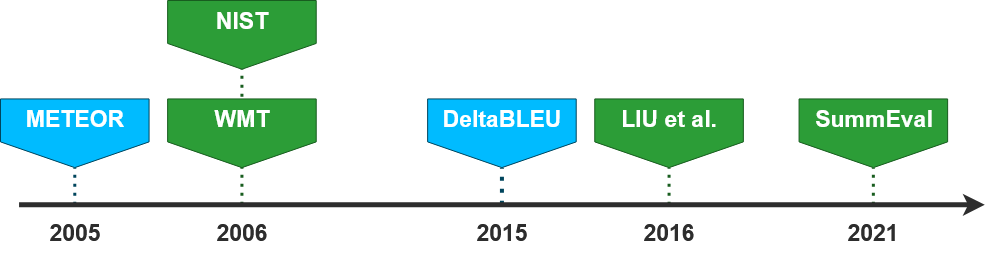
\includegraphics[width=\textwidth]{Figures/TCC-timeline-trabalhos.png}
    \end{center}
    \legend{Fonte: O autor.}
    \label{fig:timeline-treabalhos}
\end{figure}

%CONTINUA IGUAL
Em 2005, os criadores do METEOR \cite{banerjee2005meteor} realizaram uma comparação entre a sua técnica e BLEU \cite{papineni2002bleu}, demonstrando superioridade de correlação com julgamentos humanos. Com essas duas novas métricas voltadas para tradução, diversos novos trabalhos, como é o caso das campanhas realizadas por \citet{nist2006nist} e WMT \cite{koehn2006manual}, começaram a surgir a fim de comparar sistematicamente as métricas mais populares na área de tradução com anotações humanas coletadas.

Um bom tempo depois, por volta de 2015, começaram a surgir análises para outras \textit{open-ended tasks}, como sumarização e geração de diálogos. Destaca-se nesse período o trabalho que introduz o deltaBLEU \cite{galley2015deltableu}, uma métrica inspirada em BLEU \cite{papineni2002bleu} que usa pesos derivados de avaliações humanas. Além disso, nessa mesma época estudos como \textit{How NOT To Evaluate Your Dialogue System: An Empirical Study of Unsupervised Evaluation Metrics for Dialogue Response Generation} \cite{liu2016how} demonstraram correlações baixíssima entre métricas tradicionais e a avaliação humana. 

Todos esses anos de evolução culminaram em \textit{benchmarks} dedicados, como é o caso do SummEval \cite{fabbri2021summeval}, um trabalho que consolidou a prática de comparar métricas em múltiplas dimensões, influenciando até hoje trabalhos nesse campo de pesquisa.

\section{SummEval}
\label{sec:summeval}
SummEval \cite{fabbri2021summeval} foi um estudo que investigou a correlação entre os resultados obtidos através de métricas automáticas de avaliação de resumos e do julgamento humano. Para essa análise, o projeto dividiu a avaliação de cada resumo em quatro dimensões de qualidade: coerência, fluência, relevância e consistência; buscando capturar da melhor maneira possível as diferentes características que afetam a qualidade de um resumo.

Esse trabalho testou uma grande diversidade de métricas, e apontou que métricas baseadas em $n$-gramas \cite{shannon1948mathematical}, como ROUGE \cite{lin2004rouge} e BLEU \cite{papineni2002bleu} apresentam uma baixa correlação com a percepção humana, enquanto métrica baseadas em PLMs apresentam melhores resultados, mas ainda ficando aquém de capturar todas as nuances e aspectos presentes na avaliação humana.

O trabalho realizado pelos criadores do SummEval \cite{fabbri2021summeval} foi uma grande inspiração para muitos \textit{papers} na área e é inspiração direta deste trabalho como um todo.

%MUDADO (Seção nova)
\section{Question-Answering}
Quando tratamos de \textit{Question-Answering}, a quantidade de trabalhos nessa área de pesquisa apresentam uma queda significativa. Destacam-se os trabalhos de: \citet{krishna-etal-2021-hurdles}, que demonstrou que a métrica ROUGE-L não é tão informativa para esse tipo de tarefa, podendo ser facilmente burlada; \citet{han-etal-2024-rag}, que propôs três dimensões de qualidade para a avaliação desse tipo de tarefa; e \citet{farea2025evaluation}, que traz uma avaliação geral dos sistemas de \textit{Question-Answering} existentes.

Essa é uma área de crescente importância, principalmente graças a novas técnicas como RAG \cite{lewis2020retrieval} e HyDE \cite{gao2023precise}. Contudo, existe uma lacuna na literatura sobre a correlação das métricas automatizadas e avaliação humana para esse tipo de tarefa. Este trabalho busca dar um primeiro passo para preencher essa lacuna.

\section{Nossa Proposta}
Apesar de muitos trabalhos já terem tratado da comparação entre métricas e sua correlação com a opinião humana, a grande maioria desses trabalhos é realizado para a língua inglesa. Este trabalho propõe realizar essas análises com modelos e \textit{datasets} em português. Além disso, diferentemente do SummEval \cite{fabbri2021summeval}, o presente trabalho, não foca somente na tarefa de Sumarização, mas também na tarefa de \textit{Question-Answering}, 
%MUDADO
uma tarefa cuja literatura é deficitária.

%MUDADO
Sendo assim, o objetivo final do trabalho consiste em mensurar a correlação entre diferentes métricas de avaliação automatizadas e a forma de avaliação humana no âmbito de sumarização e \textit{question-answering} sobre a língua português.

\chapter{Metodologia}
\label{cap:metodologia}
Este trabalho foi dividido em seis etapas a fim de melhor organizar e apresentar a metodologia utilizada na execução do mesmo. Um \textit{pipeline} dessa divisão pode ser visto na \autoref{fig:pipeline-tcc}. Além disso, abaixo estão expressas as etapas realizadas e maiores detalhes sobre cada uma serão apresentados nas próximas seções:
\begin{enumerate}
    \item Escolha das \textit{open-ended tasks} a serem tratadas.
    \item Produção de saídas base.%: onde foram utilizados modelos e datasets públicos para a geração de saídas a serem avaliadas.
    \item Avaliação automatizada das saídas geradas.%: fazendo uso das métricas discutidas.
    \item Seleção das tarefas a serem analisadas.%: feito através de uma sample aleatória de 80 saídas, 40 para cada open-ended task tratada.
    \item Criação dos formulários para avaliação humana.%: feito com base nas tarefas tratadas, e com critérios que serão discutidos abaixo.
    \item Comparação entre as avaliações humanas e automáticas.%:  fazendo uso de cálculos de correlação entre os grupos.
\end{enumerate}

\begin{figure}[htbp]
    \caption{\textit{Pipeline} utilizado na execução do trabalho, com as etapas de produção de saídas, avaliação automatizada, seleção de saídas, criação de formulário e a comparação entre as avaliações humanas e automatizadas.}
    \begin{center}
    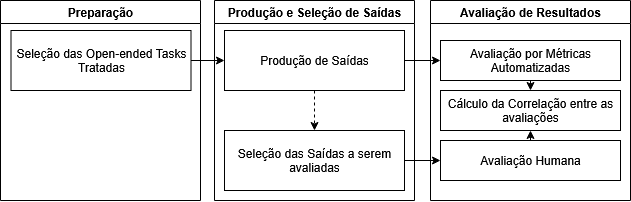
\includegraphics[width=\textwidth]{Figures/Pipeline TCC.png}
    \end{center}
    \legend{Fonte: O autor.}
    \label{fig:pipeline-tcc}
\end{figure}

\section{Tarefas Escolhidas}
As \textit{open-ended tasks} tratadas neste trabalho serão: sumarização e \textit{question-answering}. Essas duas categorias de tarefas foram escolhidas por serem tarefas comumente abordadas em trabalhos na área e possuírem problemas similares.

\subsection{Sumarização}
Se tratando de sumarização, utilizamos uma abordagem abstrativa, que busca abstrair o significado do texto base e condensá-lo em um resumo palpável. Mais informações sobre essa tarefa e possíveis abordagens podem ser vistas na \autoref{sec:summ}.

\subsection{Question-Answering}
Para esse trabalho, utilizaremos a abordagem abstrativa, pois ela é a mais aberta dentre as duas. 
%MUDADO
Contudo, a abordagem mais comumente utilizada nos dias atuais é a extrativa, dado a grande popularização de \textit{datasets} extrativos, como o SQuAD \cite{rajpurkar2016squad}. Por esse motivo, utilizaremos um \textit{dataset} mais lúdico, com intuito de permitir ao modelo uma maior liberdade de expressão, buscando tornar a tarefa o mais aberta possível. Mais informações sobre esse tipo de tarefa e suas possíveis abordagens podem ser vistas na \autoref{sec:qa}.

\section{Produção de Saídas}
\label{sec:modelos e datasets}
Em prol de facilitar a replicação dos testes e evitar introduzir um viés no uso de um \textit{dataset} autoral, ambos modelos e \textit{datasets} foram retirados de repositórios públicos. Abaixo estão descritos os modelos e \textit{datasets} escolhidos para os fins deste trabalho.

\subsection{Modelos}
\label{sec:modelos}
Para a tarefa de sumarização, o modelo utilizado foi o \textit{Portuguese T5 for Abstractive Summarization} \cite{ptt5summ_bracis}, disponibilizado no HuggingFace \footnote{Modelo Sumarização: \url{https://huggingface.co/recogna-nlp/ptt5-base-summ-xlsum}} pela Recogna \footnote{Recogna: \url{https://www.recogna.tech}}, uma empresa brasileira que atua na área de PLN. A versão do modelo escolhida foi \textit{fine-tuned} sobre o \textit{dataset} XL-Sum \cite{hasan2021xl}.

Para a tarefa de \textit{question-answering}, o modelo utilizado foi uma versão do Gemma 3 \cite{team2025gemma}, disponibilizada no HuggingFace \footnote{Modelo QA: \url{https://huggingface.co/google/gemma-3-1b-it}} pela Google DeepMind \footnote{Google DeepMind: \url{https://deepmind.google/}}. A versão escolhida possui 1 bilhão de parâmetros e foi \textit{instruction-tuned}, uma abordagem em que um modelo pré-treinado é adaptado para executar tarefas específicas, a partir de instruções fornecidas pelo usuário.

Outros modelos foram testados, contudo esses foram os modelos que apresentaram os melhores resultados em cada tarefa.

\subsection{Datasets}
\label{sec:datasets}
A língua predominante entre os \textit{datasets} da área de PLN é o inglês, por isso encontrar \textit{datasets} bem catalogados e curados para línguas divergentes é uma tarefa muito difícil. Para esse trabalho não foi diferente, a maioria dos \textit{datasets} testados apresentaram problemas, seja em erros causados por traduções diretas ou referências mal elaboradas. Após vários testes, os seguintes \textit{datasets} foram escolhidos:

Para a tarefa de sumarização, o dataset utilizado foi o \textit{CNN Dailymail Azure Pt}, disponibilizado no disponibilizado na plataforma HuggingFace \footnote{\textit{Dataset} Sumarização: \url{https://huggingface.co/datasets/arubenruben/cnn_dailymail_azure_pt_pt}} por Rúben Almeida. Esse é uma versão traduzida do \textit{dataset} \textit{CNN/DailyMail} \cite{nallapati2016abstractive}, que traz um catálogo de notícias divulgadas pelo veículo de mídia, acompanhado de sumários redigidos que são utilizados como referência para o cálculo das métricas. Esse \textit{dataset} foi escolhido pois é uma tradução do mesmo \textit{dataset} utilizado pelo SummEval \cite{fabbri2021summeval} o que permite uma melhor comparação dos resultados obtidos nesse trabalho, com os obtidos pelo SummEval.

Para a tarefa de \textit{question-answering}, o \textit{dataset} utilizado foi o \textit{FairytaleQA Translated Pt}, disponibilizado no HuggingFace \footnote{\textit{Dataset} QA: \url{https://huggingface.co/datasets/benjleite/FairytaleQA-translated-ptBR}} por Bernardo Leite. Esse \textit{dataset} foi criado a partir da tradução automática do \textit{dataset} \textit{open-source} \textit{FairytailQA} \cite{xu2022fairytaleqa}, que contém um compilado de contos de fadas curtos, além de perguntas relacionadas a cada conto e a resposta esperada para cada pergunta. Ele foi escolhido, dentre os \textit{datasets} disponíveis para língua portuguesa, por possuir um tom mais lúdico, permitindo respostas mais abstrativas quando comparado à maioria dos demais, que tendem a seguir o padrão do SQuAD \cite{rajpurkar2016squad}, que propõe uma abordagem extrativa.

\section{Métricas de Avaliação Automática}
\label{sec:métricas-metodologia}
As métricas que serão avaliadas no trabalho estão descritas na \autoref{tbl:métricas}. Para mais informações sobre as métricas, cheque as Seções \ref{sec:métricas baseadas em n-gramas} e \ref{sec:métricas baseadas em PLMs}.

\begin{table}[htbp]
    \caption{Descrição das métricas utilizadas}
    \centering
        \begin{tabular}{l c c c}
          \hline
          \textit{Métrica}  &   \textit{Baseada em}  &     \textit{Ano Criação} \\
          \hline
          \hline
          BLEU       & $n$-gramas & 2002 \\
          ROUGE      & $n$-gramas & 2004 \\
          METEOR     & $n$-gramas & 2005 \\
          BERTScore  & PLMs       & 2019 \\
          MoverScore & PLMs       & 2019 \\
          BARTScore  & PLMs       & 2021 \\
          \hline
        \end{tabular}
    \legend{Fonte: O autor.}
    \label{tbl:métricas}
\end{table}

As métricas BLEU \cite{papineni2002bleu}, METEOR \cite{banerjee2005meteor} e BERTScore \cite{bert-score}, foram implementadas através da biblioteca \textit{evaluate} disponibilizada no HuggingFace\footnote{\textit{Evaluate}: \url{https://huggingface.co/docs/evaluate/index}}. As implementações de BARTScore \cite{yuan2021bartscore} e MoverScore \cite{zhao2019moverscore} foram retiradas de seus respectivos repositórios\footnote{BARTScore: \url{https://github.com/neulab/BARTScore}}\footnote{MoverScore: \url{https://github.com/AIPHES/emnlp19-moverscore}}. Por fim, o ROUGE \cite{lin2004rouge} foi implementado através de sua biblioteca homônima\footnote{ROUGE: \url{https://pypi.org/project/rouge/}}.

Além do BLEU padrão, também foram utilizados BLEU-1 e BLEU-2, que trabalham com unigramas e bigramas, respectivamente. Essa escolha se deu pelo fato de parte das saídas serem relativamente curtas, especialmente se tratando de tarefas de \textit{question-answering}, o que favorece o uso de tais versões sobre a padrão. Já para o ROUGE, foram utilizados ROUGE-1, ROUGE-2 e ROUGE-L. Enquanto para o BERTScore, foram disponibilizados os valores de precisão, \textit{recall} e \textit{f1-score}.

\subsection{Modelos de Linguagem Pré-treinados Utilizados}
O modelo BERT \cite{devlin2019bert} utilizado para o BERTScore foi o modelo padrão definido pela biblioteca \textit{evaluate} quando a linguagem é configurada para o português, que é um modelo mBERT-base. Já para o MoverScore, o modelo utilizado foi o BERTimbau \cite{souza2020bertimbau}, disponibilizado no HuggingFace\footnote{BERTimbau: \url{https://huggingface.co/neuralmind/bert-large-portuguese-cased}} pela NeuralMind\footnote{NeuralMind: \url{https://neuralmind.ai/}}, que é pré-treinado no português brasileiro, com a versão específica utilizada sendo a versão \textit{large}. Por fim, o modelo BART \cite{lewis2019bart} utilizado para o BARTScore foi o modelo padrão presente no repositório do trabalho original. 

%MUDADO (Seção nova)
\subsection{Barreiras Linguísticas}
A implementação utilizada da métrica METEOR foi desenvolvida para o inglês, o que pode ter impactado os resultados obtidos pela mesma, já que ela faz uso de sinônimos, que não puderam ser tão aproveitados na análise para a língua portuguesa. Além disso, o modelo BART utilizado também foi treinado na língua inglesa, o que com certeza gerou resultados menos confiáveis. Contudo, os resultados apresentados por ambas as técnicas ainda foram equivalentes aos apresentados pelas demais. Possivelmente pela capacidade desses modelos de aprender e abstrair padrões linguísticos, mesmo em línguas diferentes da língua em que foram treinados.


\section{Seleção de Saídas Analisadas}
A seleção de saídas a serem analisadas se deu de forma completamente aleatória, a fim de evitar a introdução de viés. Foi feito uma amostragem randômica de 40 saídas distintas para cada tarefa, as quais foram tratadas e disponibilizadas aos participantes para avaliação, conforme descrito na próxima seção.

\section{Avaliação}
\label{sec:avaliacao-humana}
Em prol de avaliar o desempenho das métricas automatizadas discutidas na \autoref{sec:métricas-metodologia}, utilizamos avaliações humanas como fonte de comparação. Assim, permitindo correlacionar os valores obtidos através das métricas com a forma de julgamento humana. Na coleta de avaliações, humanas fizemos uso das quatro dimensões de qualidade utilizadas no \textit{paper} SummEval \cite{fabbri2021summeval}, sendo elas:

\begin{enumerate}
    \item Coerência: Qualidade geral do texto.
    \item Consistência: Alinhamento entre a saída e o texto base.
    \item Fluência: Qualidade das frases geradas.
    \item Relevância: Pontos chave selecionados para o texto.
\end{enumerate}

Contudo, no escopo deste trabalho, a dimensão de fluência foi substituída por uma dimensão de naturalidade. 
%MUDADO
Essa mudança foi realizada pois a avaliação humana não foi realizada com especialistas, o que dificulta a análise precisa da fluência de um texto, já que é necessário um grande conhecimento linguístico para se avaliar fluência. 
%CONTINUA IGUAL
A categoria naturalidade foi escolhida por ser relativamente compatível com fluência, enquanto sendo de muito mais fácil avaliação por leigos.

%MUDADO
Não existem métricas consolidadas focadas na tarefa de \textit{Question-Answering}. Por esse motivo, fizemos uso das mesmas métricas utilizadas para a Sumarização. Entendemos que nem todas as métricas se traduzem diretamente para essa tarefa, mas precisávamos de uma \textit{baseline} para as avaliações e consideramos que manter um padrão seria mais válido do que propor uma distinção sem os conhecimentos específicos de um especialista. Outrossim, acreditamos que utilizar essas dimensões, mesmo que as mesmas não tenham sido especificamente propostas para essa tarefa, seja mais válido do que apenas requisitar uma nota geral para a resposta. Afinal, essa abordagem permite uma avaliação mais clara dos erros e acertos de cada modelo.

\subsection{Coleta de Avaliações}
A coleta das avaliações humanas ocorreu através de dois formulários, cada um focado em uma das tarefas, sendo cada tarefa divida em dois grupos com vinte saídas cada. Os formulários foram então passados para oito pessoas, com quatro pessoas responsáveis por cada grupo. Para definir a nota final de uma saída é realizada uma média simples entre as notas fornecidas pelos participantes. Mais detalhes da estrutura dos formulários podem ser vistos na \autoref{sec:forms}, enquanto informações sobre o perfil dos participantes pode ser encontradas na \autoref{sec:participantes}.

\subsection{Estruturação do Formulários}
\label{sec:forms}
Cada formulário contém 40 saídas divididas em dois grupos. A informação do grupo do participante foi passada a ele junto dos links para os formulários\footnote{Formulário Sumarização: \url{https://forms.gle/phaXje34v9fPC9zE7}}\footnote{Formulário \textit{Quetion-Answering}: \url{https://forms.gle/3zdReHqiNw25RFg57}}. O formulário, então, começa requisitando ao participante que selecione o grupo em que fora colocado. O que impactará em qual grupo de saídas serão apresentadas a ele. Cada grupo de saída possui 20 saídas, que são organizadas seguindo a \autoref{tbl:forms}. 
%MUDADO
Por fim, os participantes avaliaram cada saída, fornecendo uma nota de um a cinco para cada uma das dimensões de qualidade supracitadas. 

\begin{table}[htbp]
    \centering
    \caption{Formatação da Saída fornecida aos participantes para avaliação humana.}
        \begin{tabular}{l c c c}
          \hline
          \textit{Tarefa} & \textit{Saída} & \textit{Texto/Contexto Base} & \textit{Pergunta}\\
          \hline
          \hline
          Sumarização                 & \checkmark & \checkmark & $X$\\
          \textit{Question-Answering} & \checkmark & \checkmark & \checkmark\\
          \hline
        \end{tabular}
    \legend{Fonte: O Autor.}
    \label{tbl:forms}
\end{table}

Os formulários, bem como as respostas dos usuários podem ser encontrados no github do projeto\footnote{Github: \url{https://github.com/eduardofae/Comparativo-Metricas-OET.git}} na pasta "Formulários e Repostas".

\subsection{Perfil dos Participante}
\label{sec:participantes}
Os participantes da avaliação foram todos alunos do curso de Ciência da Computação da Universidade Federal do Rio Grande do Sul. Isso faz deles conhecedores do funcionamento geral de LLMs e familiarizados com formulários eletrônicos. Contudo, por não serem especializados na área Linguística, algumas nuances das avaliações podem ter sido perdidas durante a etapa de coleta.

\section{Correlação entre Avaliações}
\label{sec:pearson-metodologia}
A fim de avaliar o grau de alinhamento entre as métricas calculadas e as avaliações coletadas, foi utilizada a correlação de Pearson. Essa escolha se deu pelo fato dessa correlação ser adequada para dados contínuos e amplamente empregada na literatura de avaliação de métricas de linguagem natural, inclusive em \textit{benchmarks} como o SummEval \cite{fabbri2021summeval}. Por esses motivos, essa foi a ferramenta escolhida com intuito de mensurar o grau de correspondência entre as métricas testadas e as avaliações humanas coletadas. A discretização dos valores de Pearson utilizada para análise dos resultados deste trabalho pode ser vista na \autoref{tbl:pearson}. Mais detalhes sobre essa técnica são apresentados na \autoref{sec:pearson}.

\begin{table}[htbp]
    \caption{Discretização dos valores de Pearson.}
    \centering
        \begin{tabular}{c l}
          \hline
          \textit{Valores de Pearson} & \textit{Interpretação} \\
          \hline
          \hline
          0.90–1.00 & Muito forte    \\
          0.70–0.89 & Forte          \\
          0.40–0.69 & Moderada       \\
          0.10–0.39 & Fraca          \\
          0.00–0.10 & Negligenciável \\
          \hline
        \end{tabular}
    \legend{Fonte: \citet{schober2018correlation}}
    \label{tbl:pearson}
\end{table}

\chapter{Validação}
Neste capítulo, serão apresentados os experimentos realizados para quantificar a correlação entre métricas automatizadas e o julgamento humano nas tarefas de Sumarização e \textit{Question-Answering}. Ademais, os resultados obtidos serão relatados e discutidos.

\label{cap:validação}
\section{Experimentos}
O objetivo dos experimentos deste trabalho é calcular a correlação entre métricas automatizadas e a avaliação humana. Para isso, foram utilizados os modelos apresentados na \autoref{sec:modelos} para a geração de todos os casos de teste presentes nos \textit{datasets} discutidos na \autoref{sec:datasets}. As saídas obtidas foram, então, avaliadas fazendo uso das métricas automatizadas vistas nas Seções \ref{sec:métricas baseadas em n-gramas} e \ref{sec:métricas baseadas em PLMs}. 

Após isso, foi realizado um \textit{sample} de oitenta saídas, quarenta para cada tarefa tratada. Essas saídas foram transformadas em formulários que foram repassados para pessoas que se tornaram responsáveis pela análise humana, como retratado na \autoref{sec:avaliacao-humana}. Finalmente, tendo os resultados das métricas e das avaliações humanas, foi calculada a Correlação de Pearson obtida para cada par de métrica e dimensão de qualidade em cada \textit{open-ended task} trabalhada, seguindo o proposto na \autoref{sec:pearson-metodologia}.

\section{Resultados e discussão}
Abaixo apresentaremos os valores de correlação divididos por área, com a \autoref{sec:summ-results} abordando Sumarização e a \autoref{sec:qa-results} abordando \textit{Question-Answering}.

\subsection{Sumarização}
\label{sec:summ-results}
A \autoref{tbl:avg-métricas-summ} apresenta a média dos valores obtidos por cada métrica nas saídas selecionadas para avaliação. Além disso, a última coluna expressa o valor médio das notas obtidas utilizando através das avaliações humanas (AHs), separadas em cada dimensão de avaliação. Ademais, é apresentado o desvio padrão (DP) médio entre as avaliações dos participantes. Isso é, a média dos desvios padrões individuais de cada saída. 
%MUDADO
Como é possível observar, os resultados obtidos em relevância, consistência e coerência foram valores baixos. Isso é, possivelmente, uma reflexão da qualidade do modelo e \textit{dataset} utilizados.

\begin{table}[htbp]
    \caption{Valor médio atribuído por cada forma de avaliação na tarefa de Sumarização.}
    \centering
        \begin{tabular}{l c c}
          \hline
          \textit{Métrica} & \textit{Valor Médio} & \textit{DP Médio}\\
          \hline
          \hline
          ROUGE-1 & 0.22 & -\\
          ROUGE-2 & 0.05 & -\\
          ROUGE-L & 0.19 & -\\
          BLEU    & 0.01 & -\\
          BLEU-1  & 0.23 & -\\
          BLEU-2  & 0.09 & -\\
          METEOR  & 0.18 & -\\
          \hline
          BERTScore-p  &  0.71 & -\\
          BERTScore-r  &  0.71 & -\\
          BERTScore-f1 &  0.71 & -\\
          BARTScore    & -3.26 & -\\
          MoverScore   &  0.61 & -\\
          \hline
          Consistência (AH) & 2.39 & 0.87\\
          Naturalidade (AH) & 3.58 & 0.97\\
          Relevância (AH)   & 2.46 & 0.97\\
          Coerência (AH)    & 2.59 & 0.95\\
          \hline
        \end{tabular}
    \legend{Fonte: O Autor.}
    \label{tbl:avg-métricas-summ}
\end{table}

Como é possível observar na \autoref{tbl:resultados-summ}, métricas baseadas em PLMs, em geral, apresentam uma maior correlação com a forma de avaliação humana em todas as dimensões de qualidade analisadas, com o MoverScore \cite{zhao2019moverscore} desempenhando abaixo dos demais. Isso se deve ao fato desse tipo de abordagem permitir captar de uma maneira mais profunda as relações semânticas entre textos, o que gera uma comparação mais justa entre as saídas e os textos referências fornecidos pelos \textit{datasets}.

\begin{table}[htbp]
    \caption{Valores de Pearson da tarefa de Sumarização.}
    \centering
        \begin{tabular}{l c c c c}
          \hline
          \textit{Métrica} & \textit{Consistência} & \textit{Naturalidade} & \textit{Relevância} & \textit{Coerência} \\
          \hline
          \hline
          ROUGE-1 & 0.21 & 0.29 & 0.29 & 0.24\\
          ROUGE-2 & 0.18 & 0.27 & 0.23 & 0.24\\
          ROUGE-L & 0.28 & 0.36 & 0.38 & 0.35\\
          BLEU    & 0.28 & 0.35 & 0.33 & 0.35\\
          BLEU-1  & 0.31 & 0.28 & 0.28 & 0.27\\
          BLEU-2  & 0.27 & 0.27 & 0.25 & 0.27\\
          METEOR  & 0.32 & 0.30 & 0.27 & 0.32\\
          \hline
          BERTScore-p  & 0.38 & 0.37 & 0.37 & 0.42\\
          BERTScore-r  & 0.38 & \textbf{0.40} & 0.40 & 0.39\\
          BERTScore-f1 & 0.40 & \textbf{0.40} & 0.40 & \textbf{0.43}\\
          BARTScore    & \textbf{0.42} & 0.38 & \textbf{0.44} & 0.40\\
          MoverScore   & 0.26 & 0.30 & 0.32 & 0.29\\
          \hline
        \end{tabular}
    \legend{Fonte: O Autor.}
    \label{tbl:resultados-summ}
\end{table}

Contudo, nenhuma das métricas conseguiu sequer se aproximar de um nível de correlação forte, tomando como base a discretização apresentada na \autoref{sec:pearson-metodologia}. Esse resultado já havia sido constatado pelo SummEval \cite{fabbri2021summeval} e outros trabalhos apresentados no Capítulo \ref{cap:trabalhos relacionados}. Todavia, os valores de Pearson obtidos neste trabalho são ainda menores do que os encontrados por \citet{fabbri2021summeval}. Acreditamos que isso seja referente a carências no \textit{dataset} utilizado, afinal a qualidade das métricas está diretamente relacionada à qualidade das referências presentes no \textit{dataset}.

\subsection{Question-Answering}
\label{sec:qa-results}
Na \autoref{tbl:avg-métricas-qa}, estão expressas as médias dos valores obtidos através das métricas automatizadas. Ademais, apresentamos as médias das notas obtidas pela Avaliação Humana, separadas por dimensão de qualidade. Juntamente do desvio padrão médio entre as avaliações de cada um dos quatro participante que avaliaram cada saída. 
%MUDADO
Outrossim, é possível perceber uma melhora nos resultados obtidos pelo modelo, quando comparado aos resultados da tarefa de sumarização. Isso pode ter acontecido dado ao fato de essa tarefa ser mais objetiva do que a anterior, ou graças a capacidades superiores do modelo utilizado.

\begin{table}[htbp]
    \caption{Valor médio atribuído por cada forma de avaliação na tarefa de \textit{Question-Answering}.}
    \centering
        \begin{tabular}{l c c}
          \hline
          \textit{Métrica} & \textit{Valor Médio} & \textit{DP Médio}\\
          \hline
          \hline
          ROUGE-1 & 0.34 & -\\
          ROUGE-2 & 0.22 & -\\
          ROUGE-L & 0.33 & -\\
          BLEU    & 0.18 & -\\
          BLEU-1  & 0.34 & -\\
          BLEU-2  & 0.25 & -\\
          METEOR  & 0.39 & -\\
          \hline
          BERTScore-p  &  0.79 & -\\
          BERTScore-r  &  0.80 & -\\
          BERTScore-f1 &  0.80 & -\\
          BARTScore    & -3.40 & -\\
          MoverScore   &  0.66 & -\\
          \hline
          Consistência (AH) & 3.44 & 0.80\\
          Naturalidade (AH) & 4.05 & 0.73\\
          Relevância (AH)   & 3.48 & 0.71\\
          Coerência (AH)    & 3.55 & 0.74\\
          \hline
        \end{tabular}
    \legend{Fonte: O Autor.}
    \label{tbl:avg-métricas-qa}
\end{table}

Diferente do esperado após os resultados obtidos em Sumarização, os resultados de \textit{Question-Answering} expressos na \autoref{tbl:resultados-qa}, apontam para uma igualdade maior entre a qualidade das métricas baseadas em PLMs e baseadas em $n$-gramas, com o METEOR \cite{banerjee2005meteor} se destacando. Isso acontece, pois essa tarefa, mesmo utilizando uma abordagem abstrativa, ainda é muito mais fechada do que a Sumarização, o que faz com que métricas que comparam diretamente palavras entre a saída e a referência sejam favorecidas. 
%MUDADO
Além disso, como as respostas geradas tendem a ser mais curtas, com muitas palavras extraídas do contexto, o espaço para problemas como sinônimos tende a ser menor, o que melhora o desempenho das métricas baseadas em $n$-gramas. Uma exemplificação desse comportamento pode ser vista na \autoref{fig:qa-exemplo}.

\begin{table}[htbp]
    \caption{Valores de Pearson da tarefa de \textit{Question-Answering}.}
    \centering
        \begin{tabular}{l c c c c}
          \hline
          \textit{Métrica} & \textit{Consistência} & \textit{Naturalidade} & \textit{Relevância} & \textit{Coerência} \\
          \hline
          \hline
          ROUGE-1 & 0.58 & 0.45 & 0.56 & 0.55\\
          ROUGE-2 & 0.50 & 0.33 & 0.51 & 0.49\\
          ROUGE-L & 0.56 & 0.44 & 0.55 & 0.54\\
          BLEU    & 0.43 & 0.24 & 0.44 & 0.43\\
          BLEU-1  & 0.51 & 0.37 & 0.50 & 0.49\\
          BLEU-2  & 0.53 & 0.37 & 0.53 & 0.52\\
          METEOR  & \textbf{0.61} & 0.49 & 0.59 & \textbf{0.59}\\
          \hline
          BERTScore-p  & 0.57 & 0.45 & 0.58 & 0.56\\
          BERTScore-r  & 0.59 & \textbf{0.51} & 0.60 & 0.57\\
          BERTScore-f1 & 0.60 & 0.50 & \textbf{0.61} & \textbf{0.59}\\
          BARTScore    & 0.60 & 0.48 & 0.58 & \textbf{0.59}\\
          MoverScore   & 0.44 & 0.26 & 0.44 & 0.42\\
          \hline
        \end{tabular}
    \legend{Fonte: O Autor.}
    \label{tbl:resultados-qa}
\end{table}

%MUDADO
\begin{figure}[htbp]
    \caption{Exemplo de saída para a tarefa de \textit{Question-Answering} que demonstra como, mesmo em abordagens abstrativas, as respostas tendem a ser mais curtas e com palavras extraídas do texto.}
    \begin{center}
    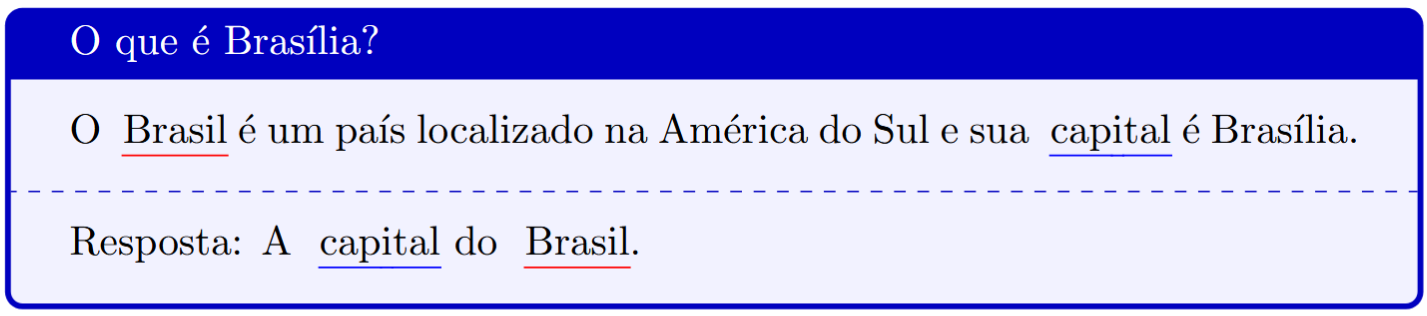
\includegraphics[width=\textwidth]{Figures/qa-2.png}
    \end{center}
    \legend{Fonte: O autor.}
    \label{fig:qa-exemplo}
\end{figure}

Contudo, apesar dos melhores resultados, nenhuma das métricas conseguiu atingir um nível de correlação forte, tomando como base a discretização apresentada na \autoref{sec:pearson-metodologia}. Como não temos uma boa \textit{baseline} para comparação, como a disponibilizada por \citet{fabbri2021summeval}, não podemos avaliar com tanta precisão o impacto causado pelo \textit{dataset} utilizado. Todavia, dado o fato de o mesmo não ser diretamente produzido para o português é possível acreditar que a qualidade do \textit{dataset} possa ter impactado nos resultados obtidos.

\subsection{Discussão}
Esses resultados apontam para uma necessidade de novas métricas que melhor se correlacionem com a percepção humana. Ademais, demonstramos como métricas baseadas em $n$-gramas podem gerar resultados superiores a métricas baseadas em PLMs em casos específicos. Contudo, é também possível perceber que, no geral, métricas baseadas em PLMs possuem uma maior correlação com a forma de avaliação humana.

Evidenciam, ainda, a carência de \textit{datasets} bem estruturados e curados na língua portuguesa. O que torna necessário, em vários casos, o uso de \textit{datasets} traduzidos e adaptados ao invés de produzidos diretamente para o português. Isso impacta diretamente nos resultados das métricas, já que a qualidade de toda métrica é diretamente dependente da qualidade das referências disponibilizadas. Afinal, caso uma referência seja incorreta, a métrica irá favorecer saídas alinhadas com o resultado errado e desfavorecer saídas alinhadas ao resultado que deveria ser correto.

\chapter{Conclusão}
\label{cap:conclusão}
Através dos resultados obtidos, este estudo conclui que a correlação entre as métricas automatizadas mais popularmente utilizadas e a avaliação humana é extremamente baixa para o esperado em anos de pesquisas na área. Isso aponta uma carência severa de novas métricas que apresentem maiores ligações com o julgamento humano. Além disso, o trabalho observou que um possível caminho possam ser as métricas baseadas em PLMs, visto que apresentam uma correlação significantemente maior do que as suas antecessoras, apesar de sua recente introdução. Ademais, esse tipo de métrica possui maior capacidade de capturar relações semânticas profundas entre as saídas e os textos de referência. Também acredita-se que é de suma importância que novos \textit{datasets} sejam produzidos inteiramente na língua portuguesa, visto que essa foi uma carência muito visível durante a etapa de seleção dos \textit{datasets} utilizados.

\section{Limitações}
As maiores limitações deste trabalho foram a dificuldade de encontrar bons \textit{datasets} na língua portuguesa. Visto que a maior parte da informação disponível no mundo digital está contida na língua inglesa, sendo ela a língua franca do mundo científico. Essa valorização da língua inglesa traz também uma desvalorização das demais línguas, dificultando muito o encontro de \textit{datasets} específicos e bem estruturados para línguas divergentes. Em sua maioria, os \textit{datasets} são feitos a partir de traduções automatizadas de \textit{datasets} originários da língua inglesa, o que acarreta em problemas quando realizado de maneira descuidada. Isso se torna um agravante ainda maior quando as referências esperadas estão mal escritas ou não são condizentes com o texto base, quando os próprios textos bases não estão bem escritos, ou quando as perguntas são mal formuladas. Todos esses problemas precisam ser levados em conta quando avaliamos a eficácia de uma métrica. Afinal, a qualidade de uma métrica é limitada à qualidade da referência em que ela se baseia.

Além disso, como a maior parte dos \textit{datasets} disponíveis online se encontram na língua inglesa, é também comum que a maior parte dos modelos seja treinado para a língua inglesa. Isso acarreta em modelos menos capazes para línguas divergentes do inglês, o que se provou uma grande limitação para esse trabalho, tanto na geração de saídas quanto no uso desses modelos em métricas baseadas em PLMs.

% Outra limitação importante é o tempo de pesquisa. A geração de boas saídas e a obtenção de avaliações por usuários leva tempo e dedicação, tanto por parte de desenvolvimento quanto por parte dos avaliadores. Ademais, com mais tempo e pesquisa, poderia-se criar um \textit{dataset} próprio, melhor estruturado e curado, o que traria resultados e análises mais confiáveis, e permitiria que outras pessoas interessadas expandissem em cima da ideia. Do mesmo modo, com mais tempo poderia-se convidar especialistas para trazer uma abordagem mais científica e especializada para as análises, permitindo até voltarmos com fluência como dimensão de qualidade, que teve de ser removida deste projeto.

\section{Trabalhos Futuros}
Esse tema está longe de ser resolvido, e este trabalho é apenas um passo nessa odisseia de correlacionar as métricas utilizadas na avaliação intrínseca com a forma de avaliação humana, especialmente no âmbito da língua portuguesa. Existem muitas métricas que não foram abordadas neste trabalho, os \textit{datasets} e modelos utilizados apresentaram inúmeras limitações e inúmeras \textit{open-ended tasks} inexploradas. Contudo, isso é apenas uma oportunidade para que novos trabalhos expandam nesse tópico tão carente de atenção. Algumas possibilidades de trabalhos futuros são:

\begin{enumerate}
    \item Desenvolvimento de um \textit{dataset} especializado.
    \item Treinamento/\textit{fine-tuning} de um modelo sobre esse novo \textit{dataset}.
    \item Testes com novas métricas.
    \item Treinamento/\textit{fine-tuning} de modelos para uso nas métricas baseadas em PLMs.
    \item Análise com uma população maior.
    \item Análise com especialistas.
    \item Desenvolvimento de novas métricas.
\end{enumerate}

%MUDADO
Além disso, alguns pontos específicos que poderiam ser melhor explorados são o uso de um modelo BART treinado especificamente para o português no BARTScore e o uso de \textit{wordnets} para sinônimos na métrica METEOR. Outro ponto importante é que os modelos BERT utilizados no BERTScore e MoverScore são diferentes, é interessante a realização de testes com o mesmo modelos, o que permitiria uma melhor comparação do desempenho de ambas métricas.

Como pode ser observado, este é um tema que ainda está muito aberto para exploração. Ademais, é de suma importância que o mesmo seja mais abordado em pesquisas, principalmente no âmbito nacional. Afinal, LLMs são atualmente uma das tecnologias mais revolucionárias já desenvolvidas e não podemos permitir que uma tecnologia com tanto potencial sofra pela carência de boas métricas para avaliação de seu desempenho.

\bibliographystyle{abntex2-alf}
\bibliography{biblio}

\end{document}
